\chapter{Implemented System}
\thispagestyle{fancy}

For the purpose of obtaining an insight into how a person who suffers from food allergies or a form of food intolerance perceives different variations of the visualization of allergens, the mobile application \emph{Allergy Scan} was developed\footnote{The entire project is publicly accessible on \emph{https://gitlab.com/michaelcamper/allergy-scan-next}}. 

\section{Application Design}

\subsection{Registration}
\label{sub:config}

On the initial launch the user is prompted with a three-step configuration process. Firstly, the user is welcomed to the application (\cref{fig:config-0}) and can define an allergy profile by marking up to 14 critical allergens (\cref{fig:config-1}). Secondly, the user fills out a form (\cref{fig:config-2}) which collects demographic and behavioral data (\cref{table:user-profiling}). Lastly, the user gets assigned randomly into one of the four test groups (\cref{sec:text-groups}). The application also concludes on the participant’s preferred language through the settings of the user’s device. 


\begin{figure}[H]
     \centering
     
     \begin{subfigure}[b]{0.28\textwidth}
         \centering
         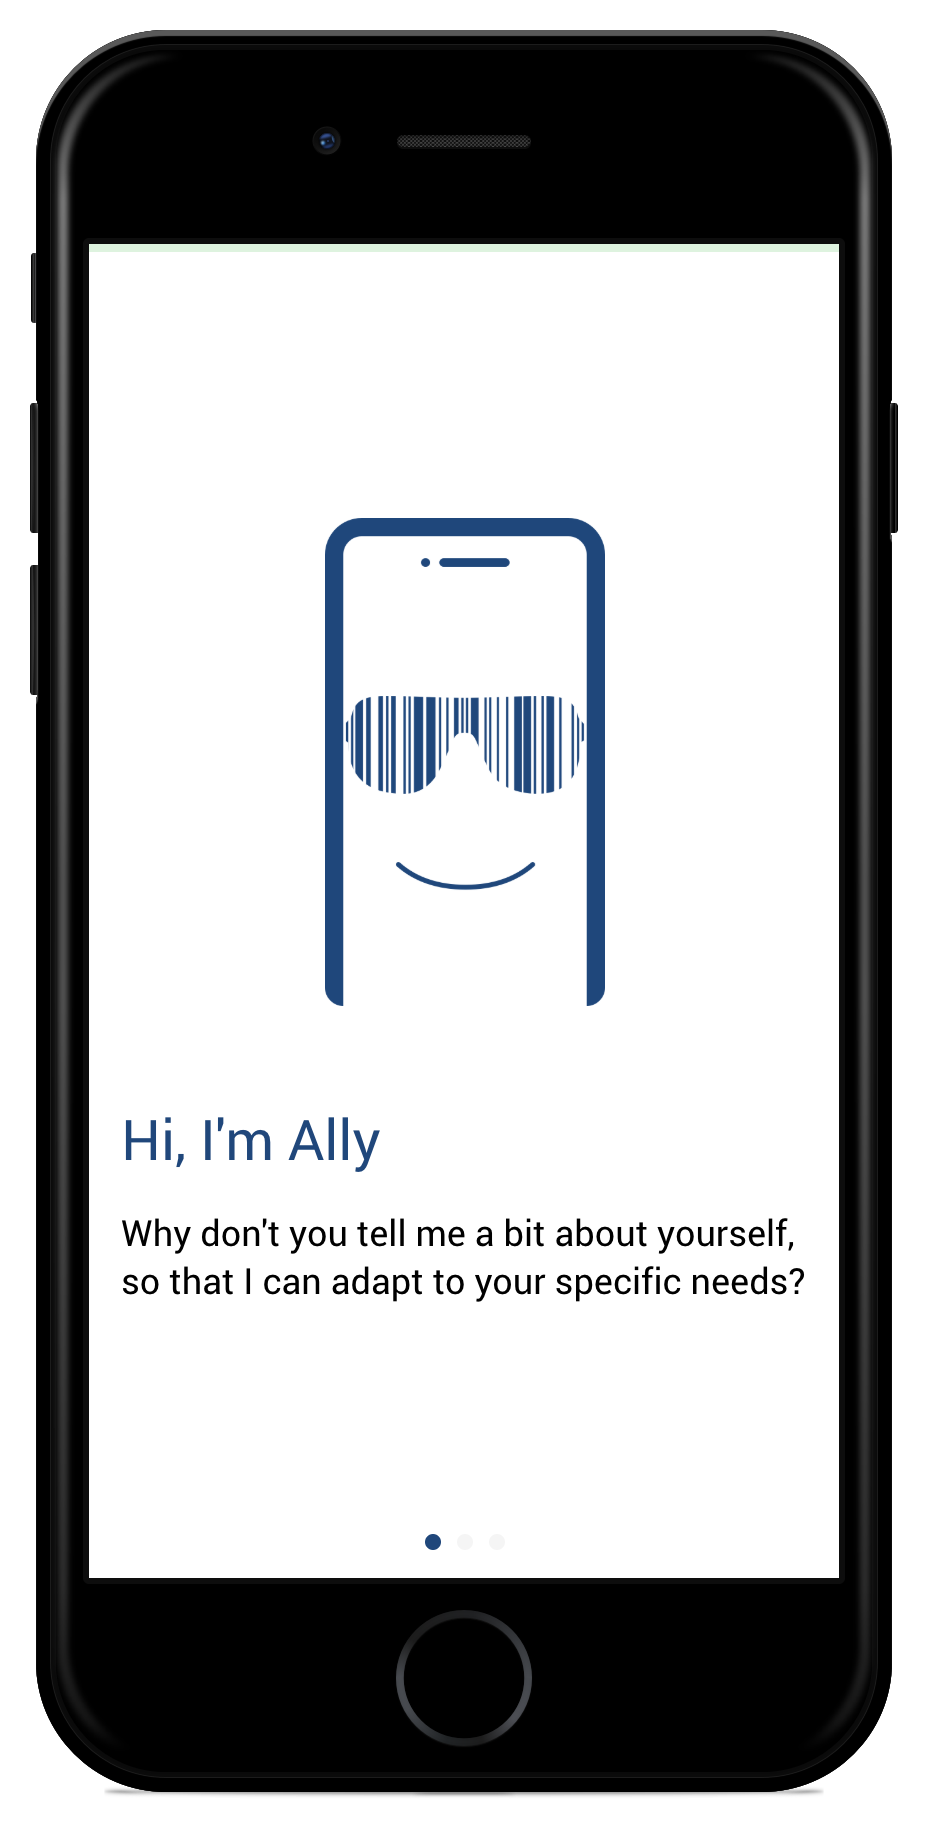
\includegraphics[width=\textwidth]{config-0}
         \caption{Welcome screen}
         \label{fig:config-0}
     \end{subfigure}
          \hfill
     \begin{subfigure}[b]{0.28\textwidth}
         \centering
         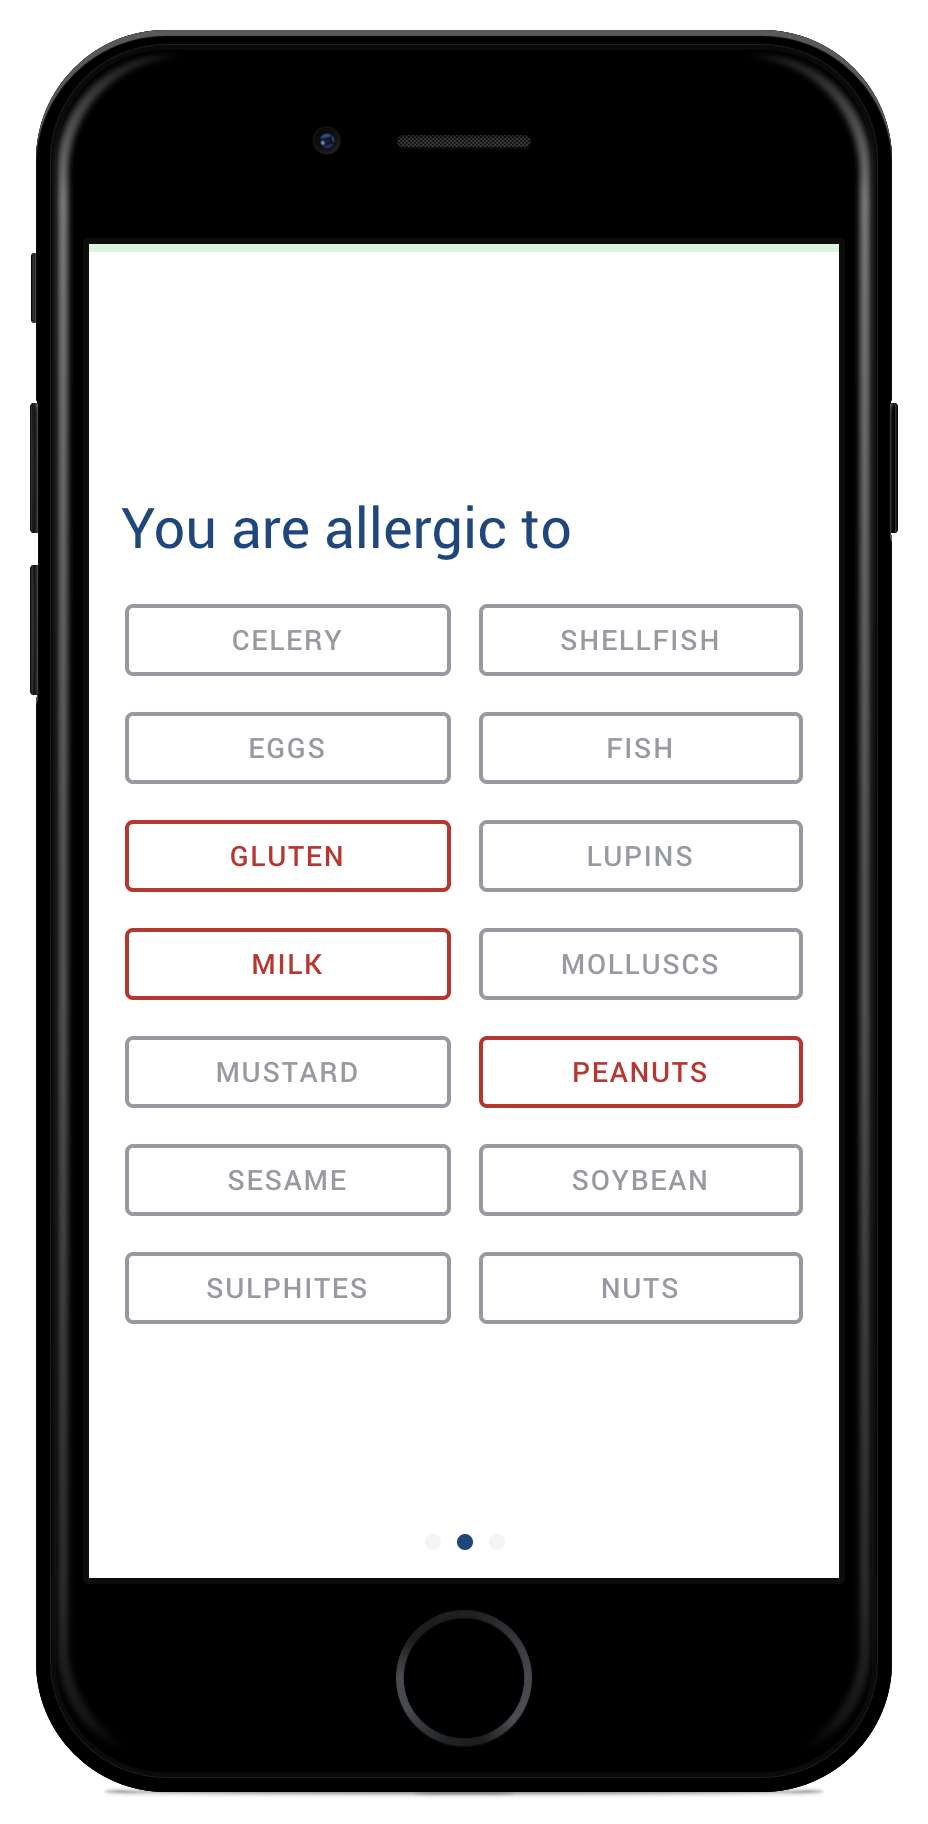
\includegraphics[width=\textwidth]{config-1}
         \caption{Allergy selector}
         \label{fig:config-1}
     \end{subfigure}
          \hfill
     \begin{subfigure}[b]{0.28\textwidth}
         \centering
         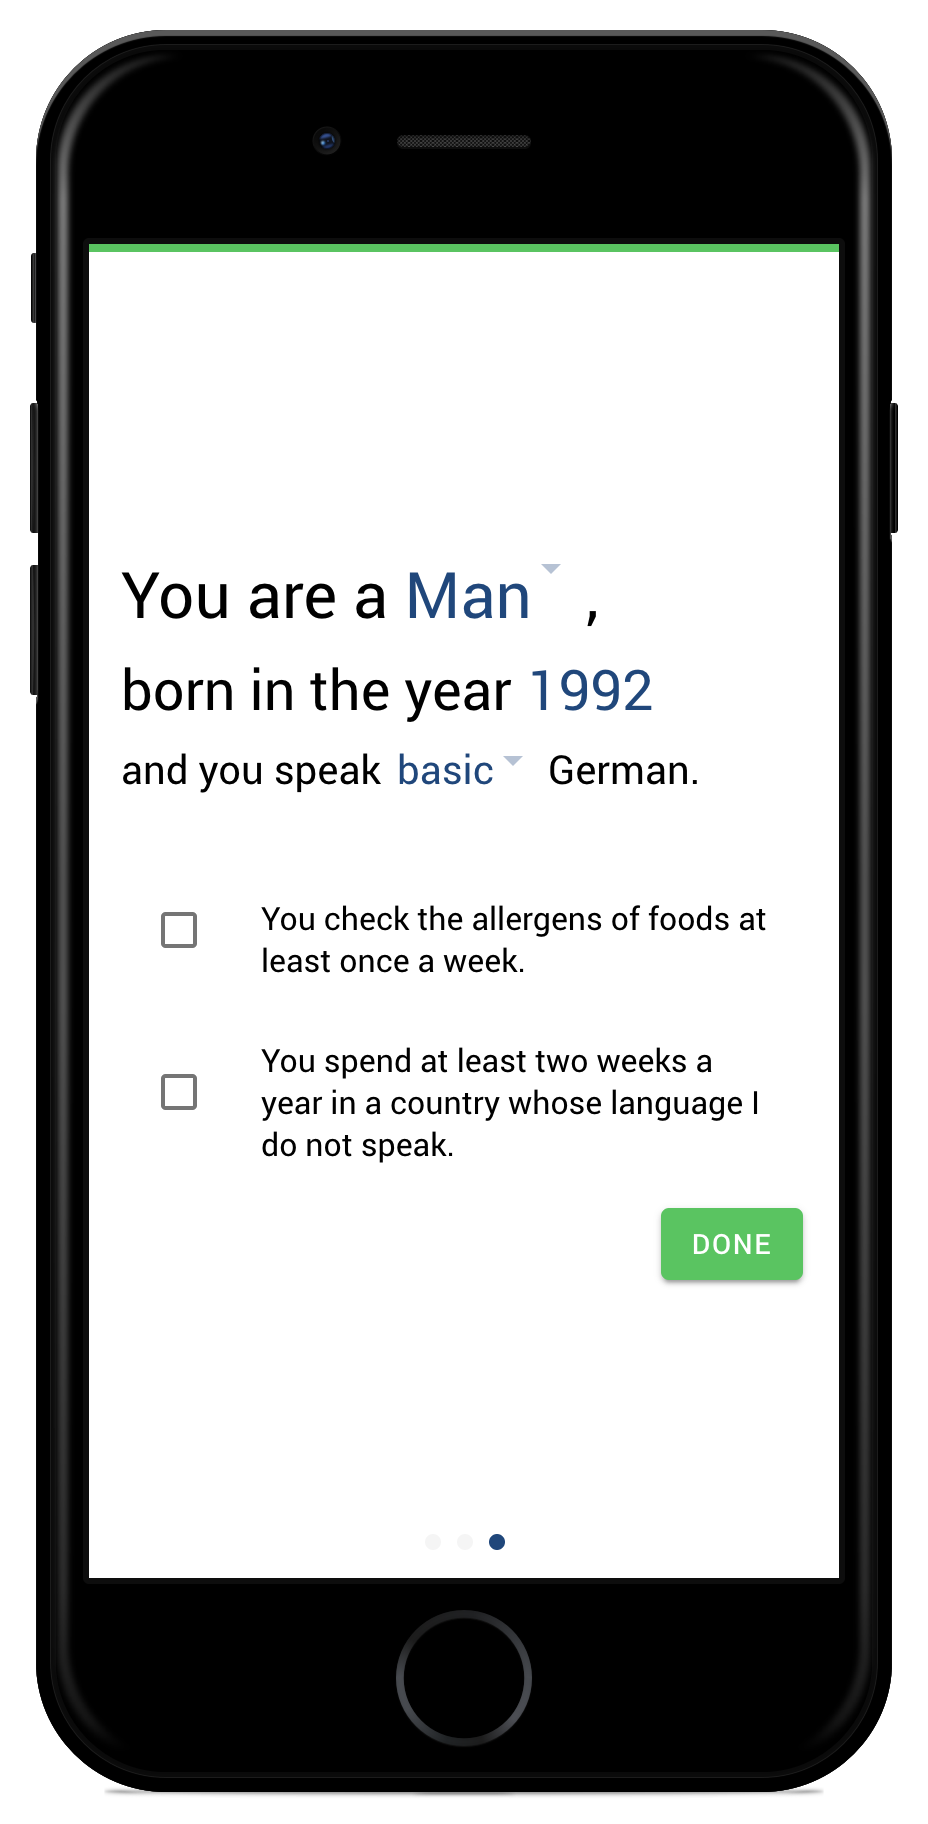
\includegraphics[width=\textwidth]{config-2}
         \caption{Registration form}
         \label{fig:config-2}
     \end{subfigure}
        \caption{Initial configuration}
        \label{fig:config}
\end{figure}

\subsection{Product Scanner}

After \emph{Allergy Scan} has launched and is configured to the user, a minimalist home screen (\cref{fig:home-0}) appears. Here, the user is able to scan a product's bar code (\cref{fig:home-1}). This bar code is parsed and sent to the Eatfit API (\cref{sub:eatfit}). Depending on whether the product can be successfully retrieved from Eatfit's database, the information about the product will either be displayed immediately after the successful scan (\cref{sub:result}) or the user will be asked to capture the missing product (\cref{sub:capture}). Each product scan is stored (\cref{table:user-behavior}) and the history can be accessed by the user (\cref{fig:home-2}).

\begin{figure}[H]
     \centering
     
     \begin{subfigure}[b]{0.28\textwidth}
         \centering
         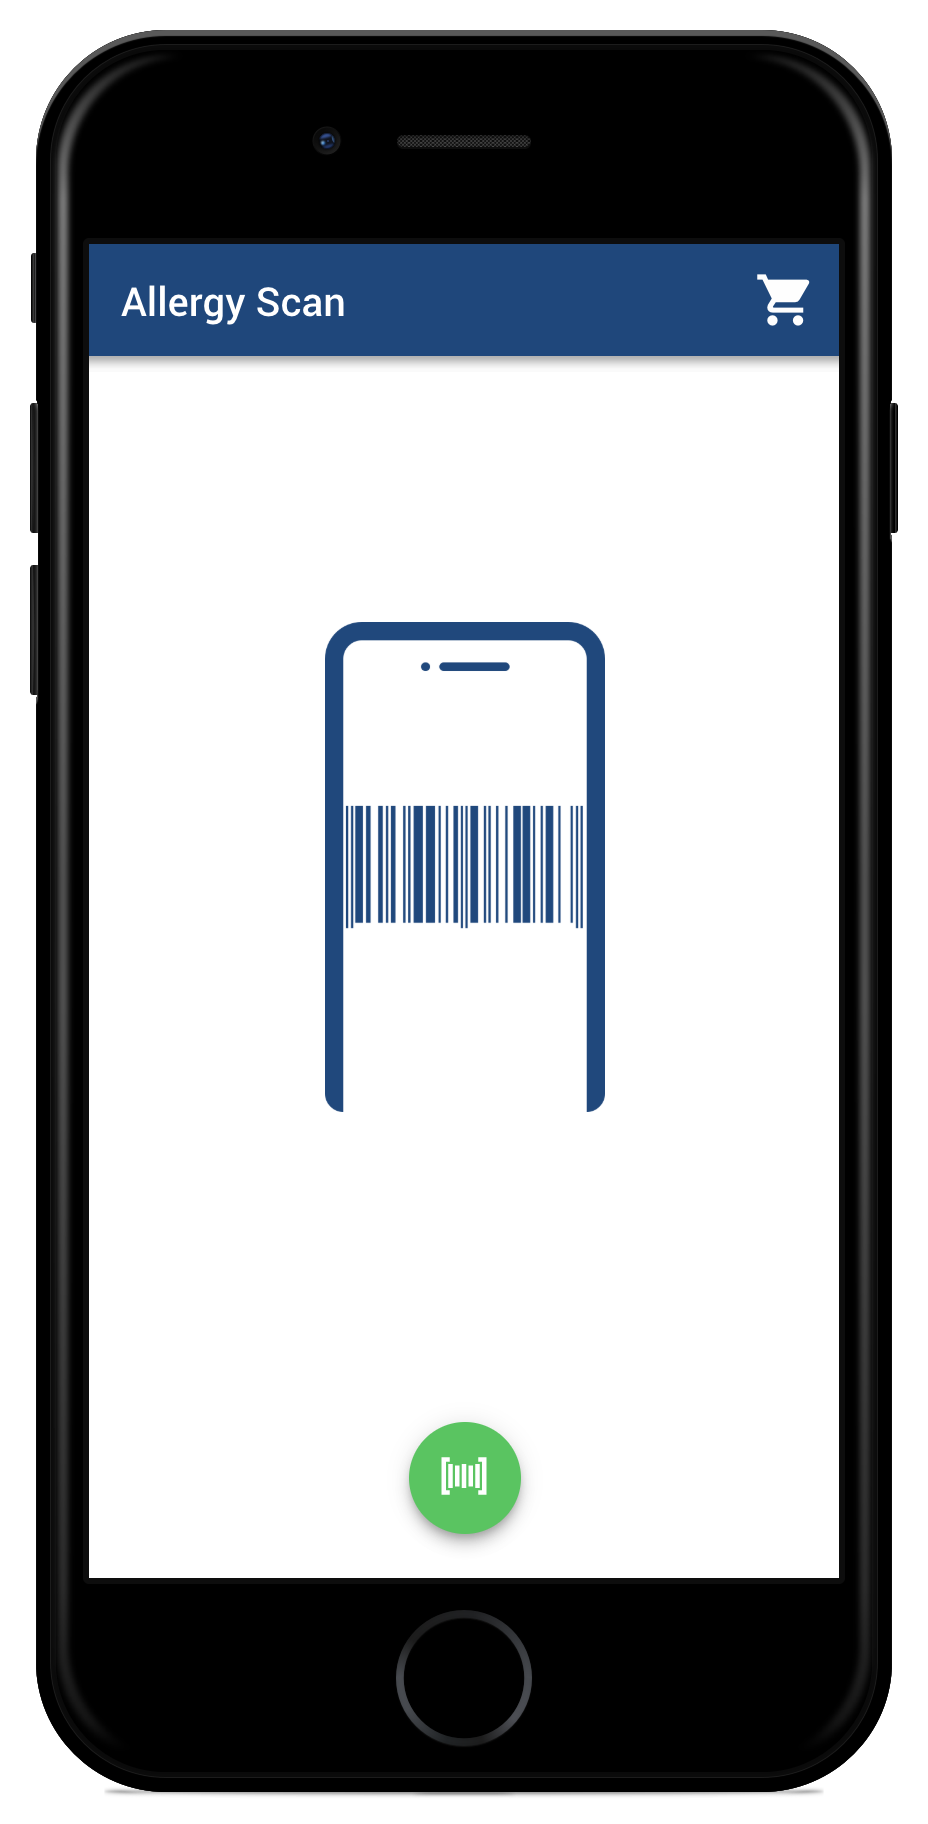
\includegraphics[width=\textwidth]{home-0}
         \caption{Home screen}
         \label{fig:home-0}
     \end{subfigure}
          \hfill
     \begin{subfigure}[b]{0.28\textwidth}
         \centering
         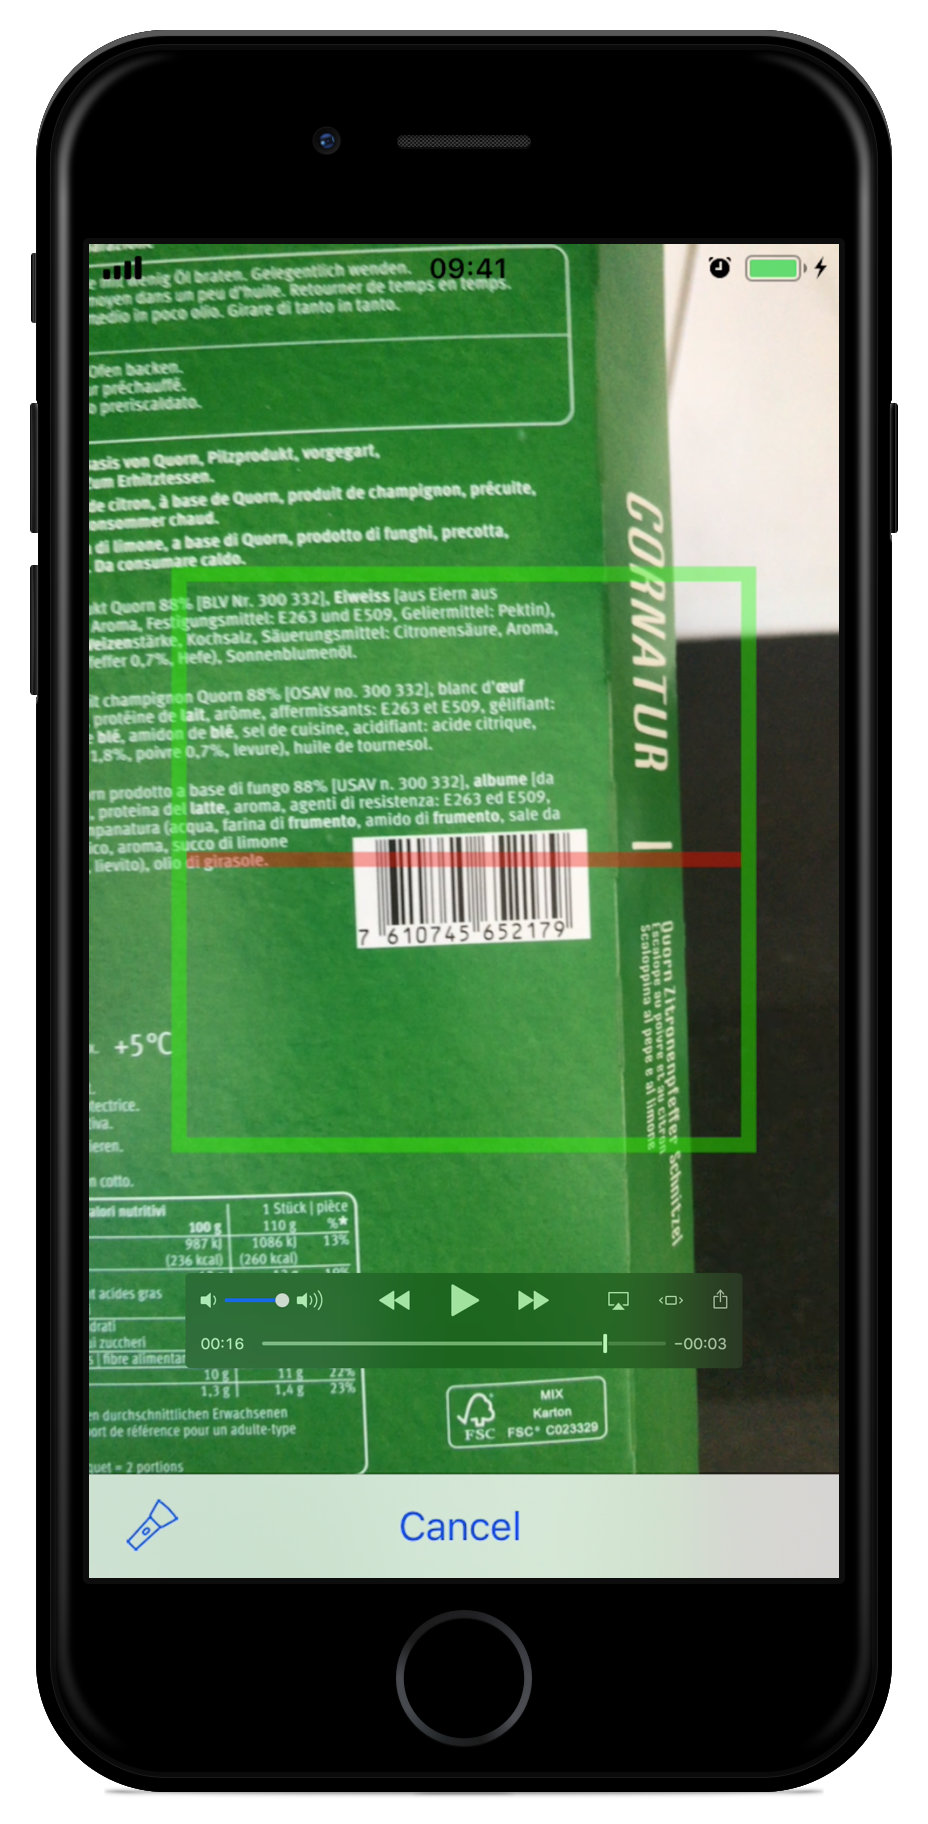
\includegraphics[width=\textwidth]{home-1}
         \caption{Scanning a product}
         \label{fig:home-1}
     \end{subfigure}
          \hfill
     \begin{subfigure}[b]{0.28\textwidth}
         \centering
         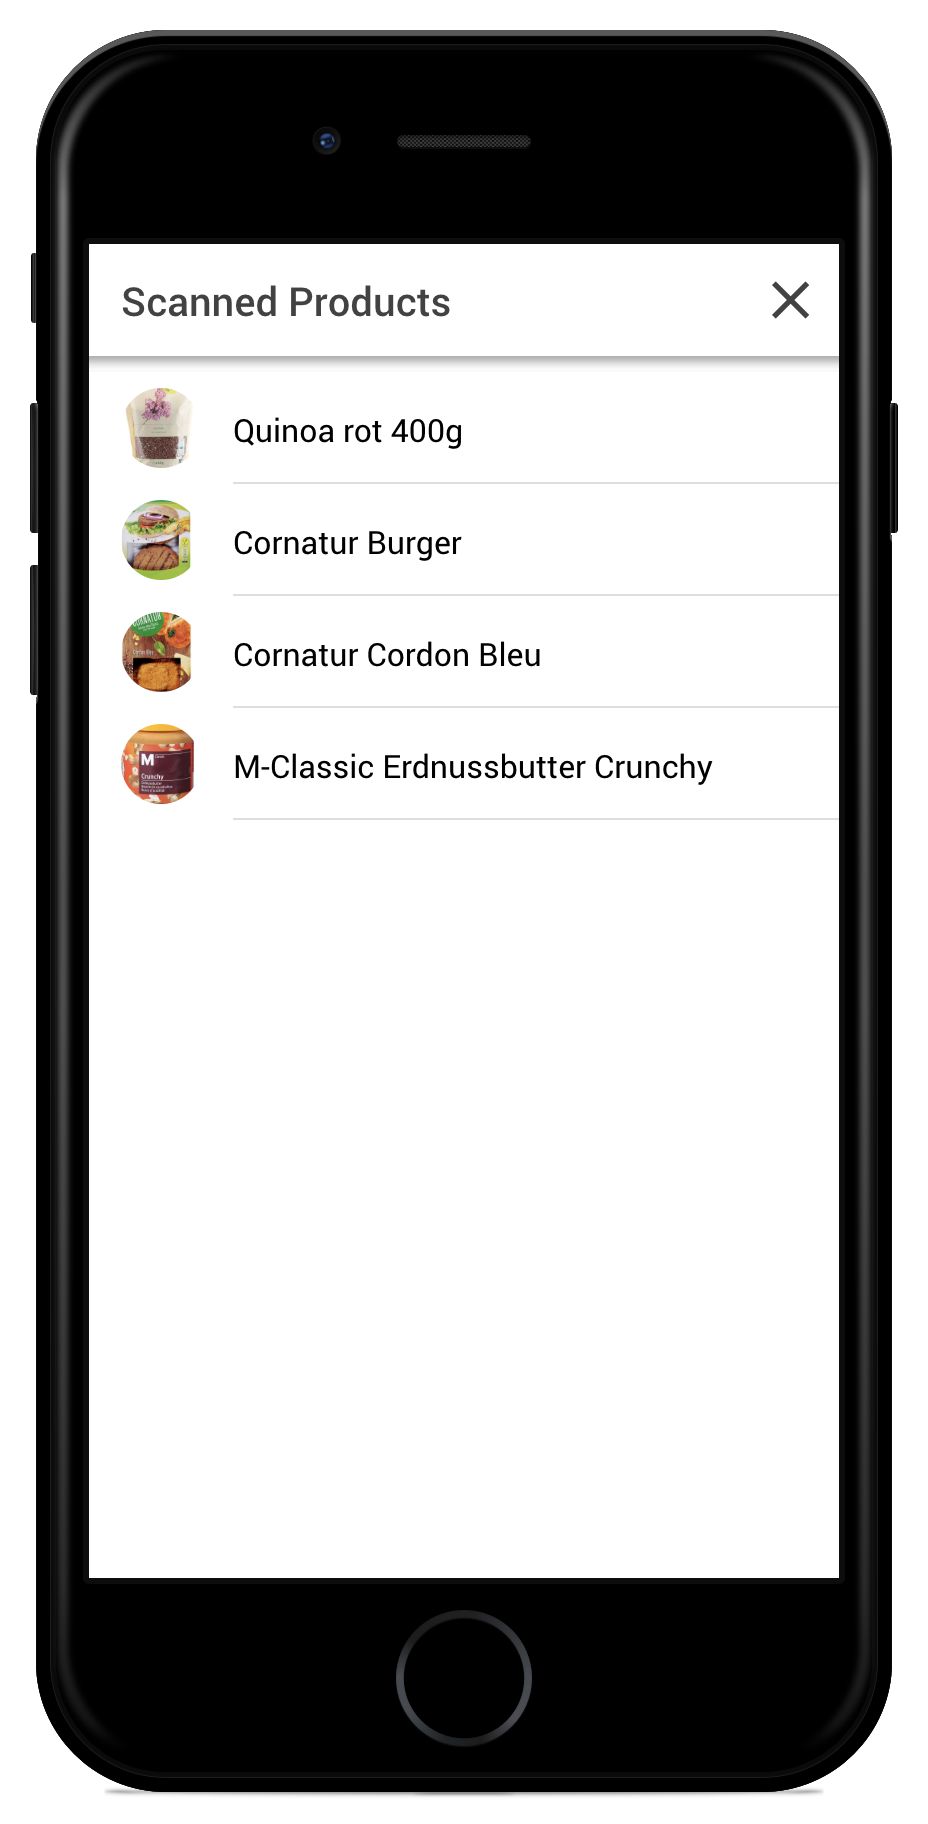
\includegraphics[width=\textwidth]{home-2}
         \caption{Scan history}
         \label{fig:home-2}
     \end{subfigure}
        \caption{Core functionality}
        \label{fig:home}
\end{figure}

\subsection{Result View}
\label{sub:result}

The information about the food item will be displayed after the product is scanned and retrieved successfully from the database. This is the point where the A/B-Testing (\cref{sec:text-groups}) is applied. Depending on which test group the user is assigned to, the presentation of the contained allergens will be different. If the user is assigned to a \emph{non-tailored} test group, all allergens that the food item contains are shown (\cref{fig:result-ni} and \cref{fig:result-nt}), or else, only the allergens which are critical to the user are displayed (\cref{fig:result-ti} and \cref{fig:result-tt}). If the user is allocated to a \emph{visual} test group the allergens are presented as icons (\cref{fig:result-ti} and \cref{fig:result-ni}), otherwise the allergens will appear in the form of a text (\cref{fig:result-tt} and \cref{fig:result-nt}).

\begin{figure}[H]
     \centering
     \begin{subfigure}[b]{0.2\textwidth}
         \centering
         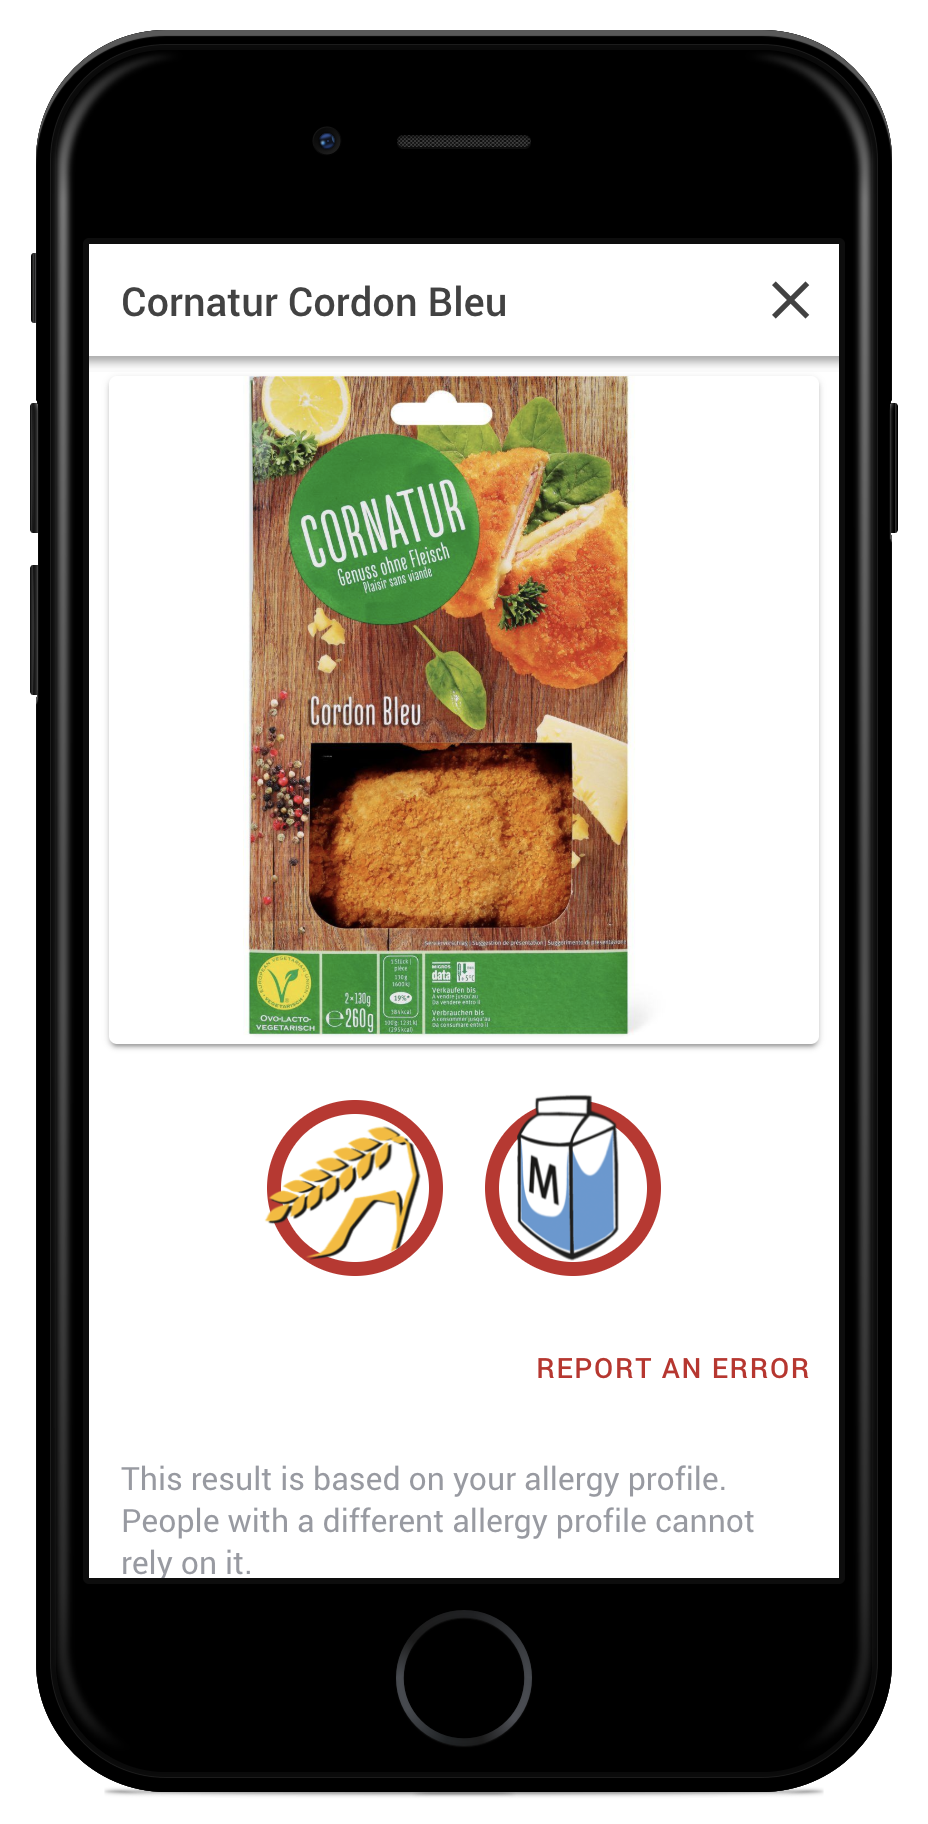
\includegraphics[width=\textwidth]{result-ti}
         \caption{Tailored\linebreak Visual}
         \label{fig:result-ti}
     \end{subfigure}
          \hfill
     \begin{subfigure}[b]{0.2\textwidth}
         \centering
         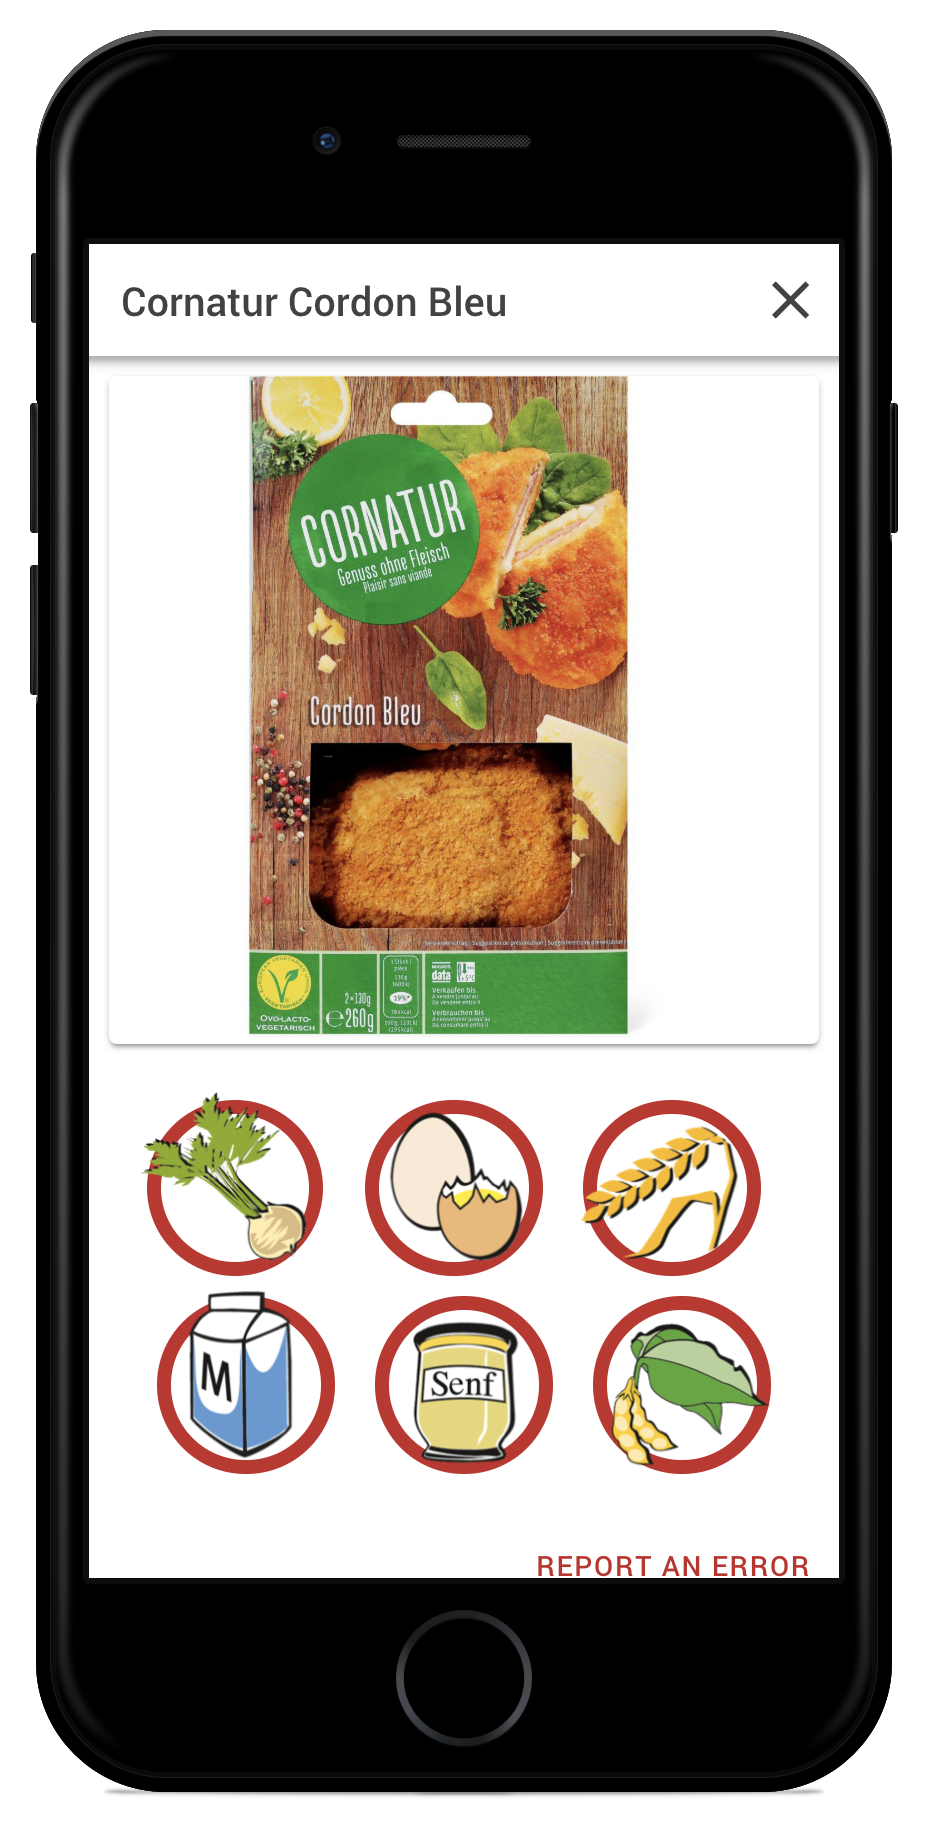
\includegraphics[width=\textwidth]{result-ni}
         \caption{Non-tailored\linebreak Visual}
         \label{fig:result-ni}
     \end{subfigure}
          \hfill
     \begin{subfigure}[b]{0.2\textwidth}
         \centering
         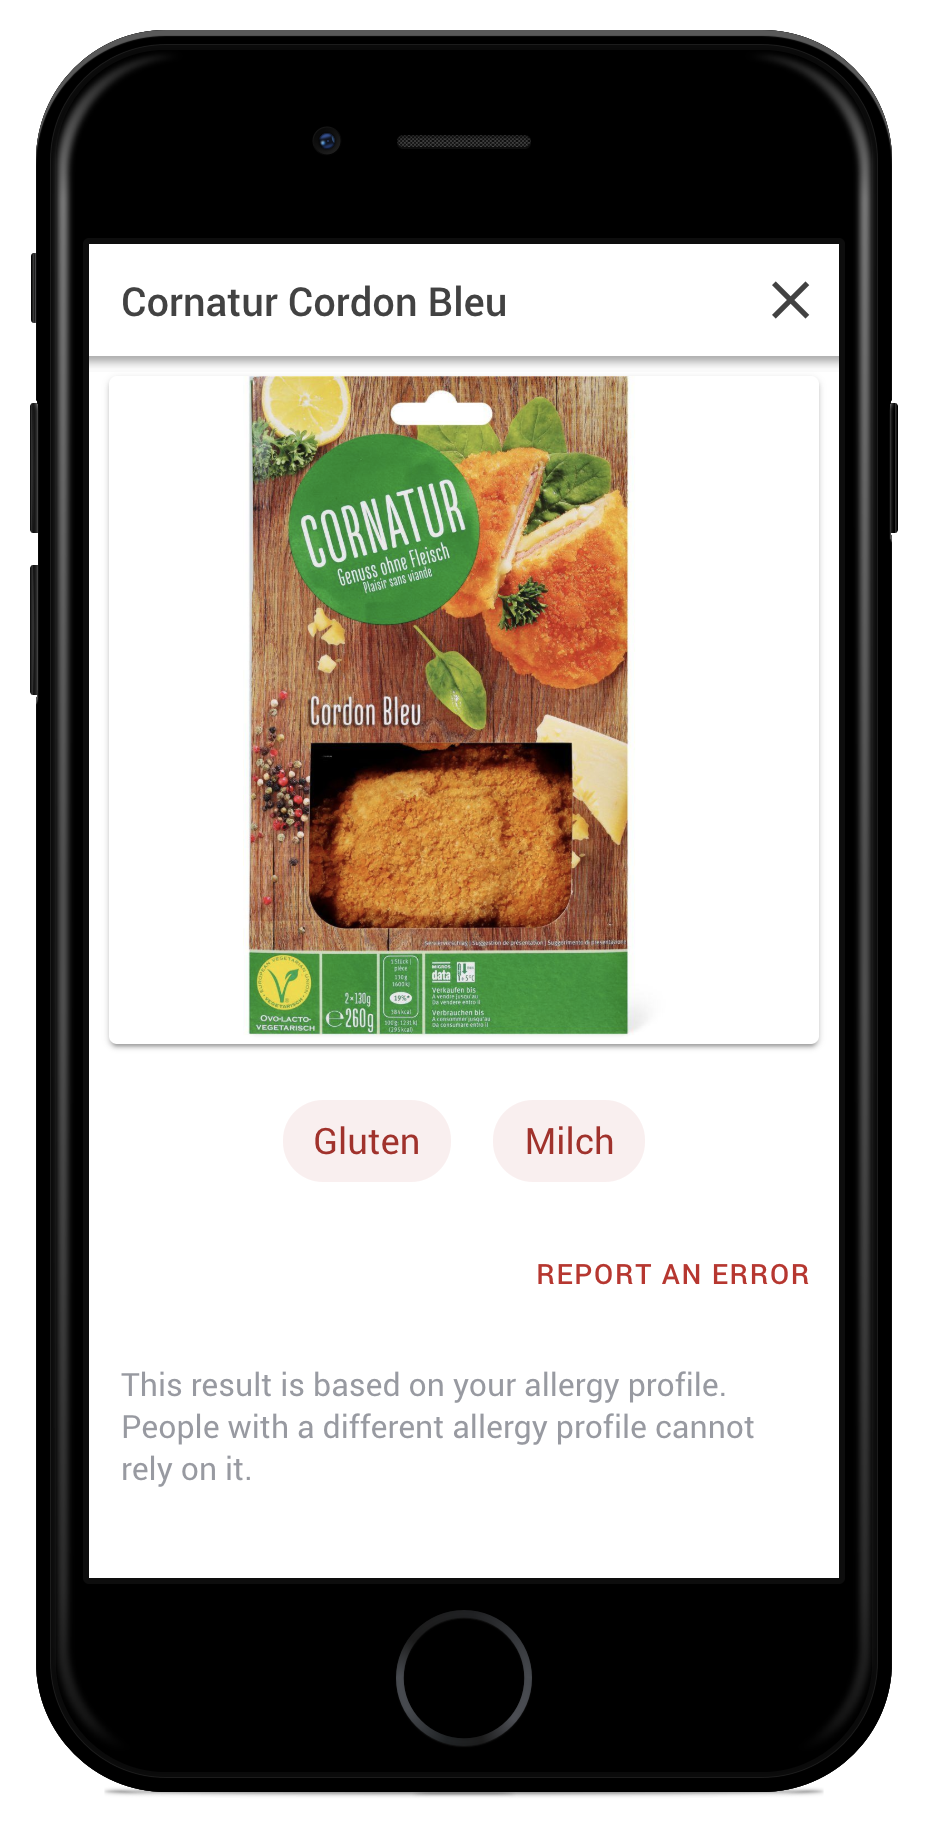
\includegraphics[width=\textwidth]{result-tt}
         \caption{Tailored\linebreak Textual}
         \label{fig:result-tt}
    \end{subfigure}
          \hfill
     \begin{subfigure}[b]{0.2\textwidth}
         \centering
         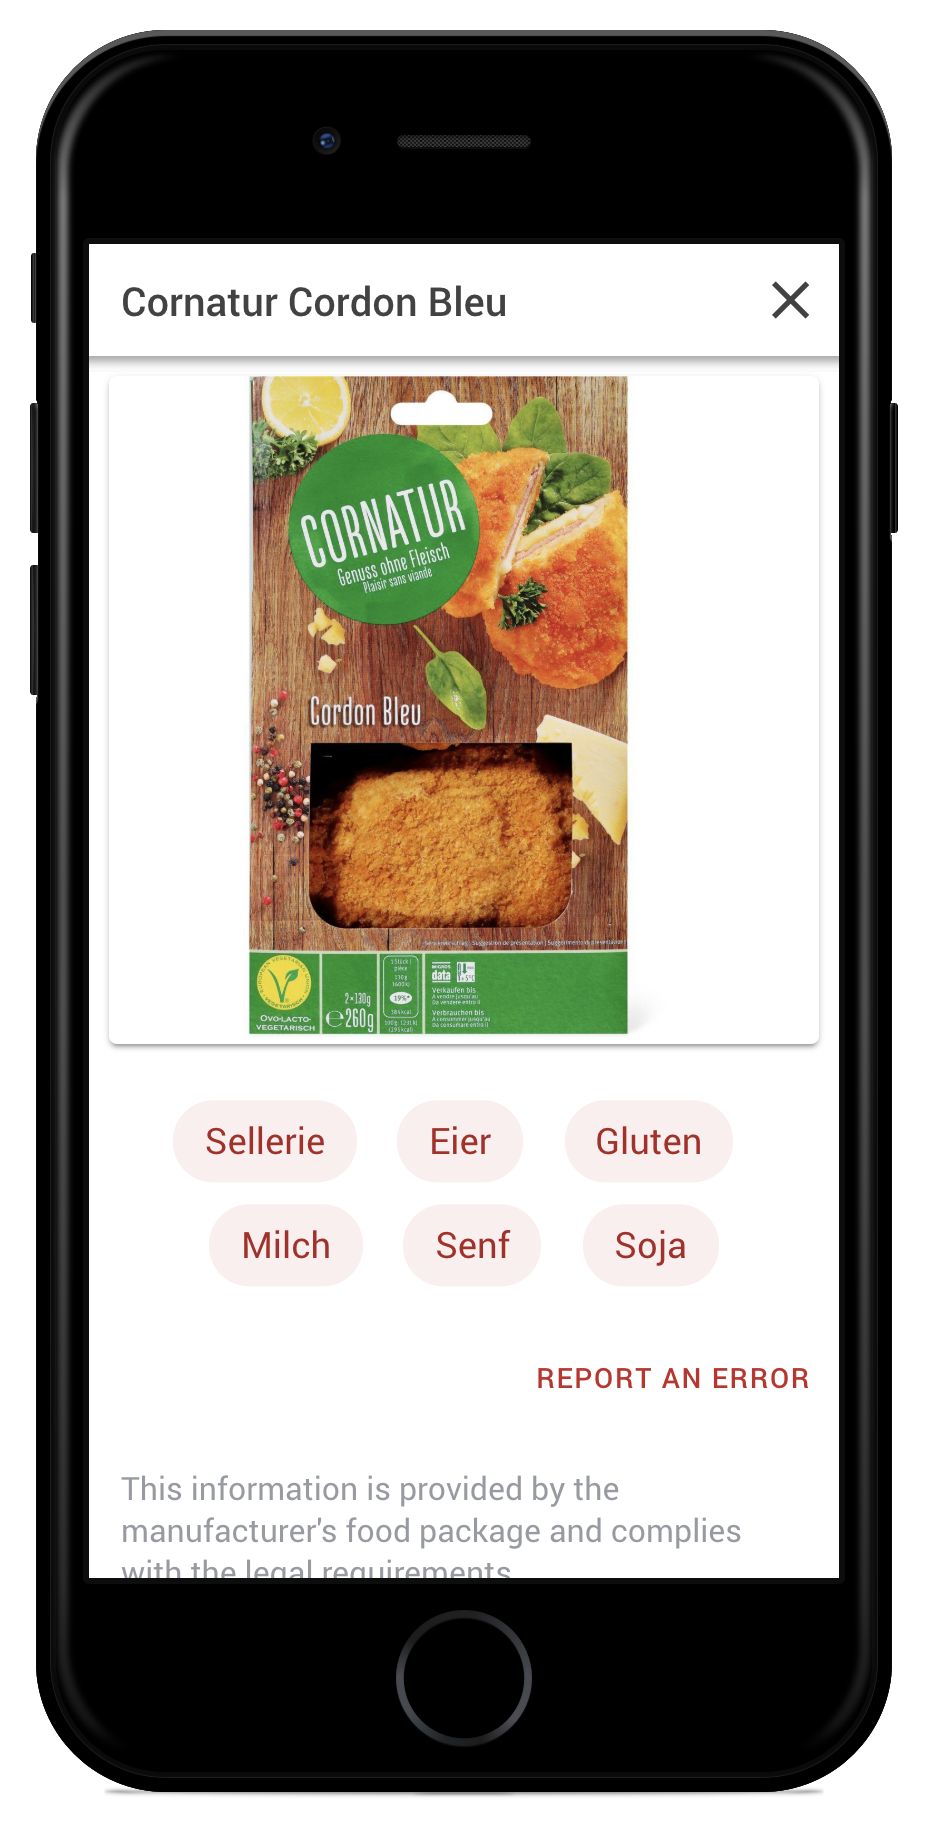
\includegraphics[width=\textwidth]{result-nt}
         \caption{Non-tailored\linebreak Textual}
         \label{fig:result-nt}
     \end{subfigure}
        \caption{Result presentation by test group}
        \label{fig:result}
\end{figure}

\subsection{Product Capture}
\label{sub:capture}

In case that the product is not found on Eatfit's database, the user is asked to voluntarily capture the product, so that the missing product will be made available for other users in the future. The user must capture the name of the product (\cref{fig:capture-0}), take a proper photo of the whole product for representational purposes (\cref{fig:capture-1}) and photograph the list of ingredients, which delivers information on the contained allergens (\cref{fig:capture-2}).

\begin{figure}[H]
     \centering
     \begin{subfigure}[b]{0.28\textwidth}
         \centering
         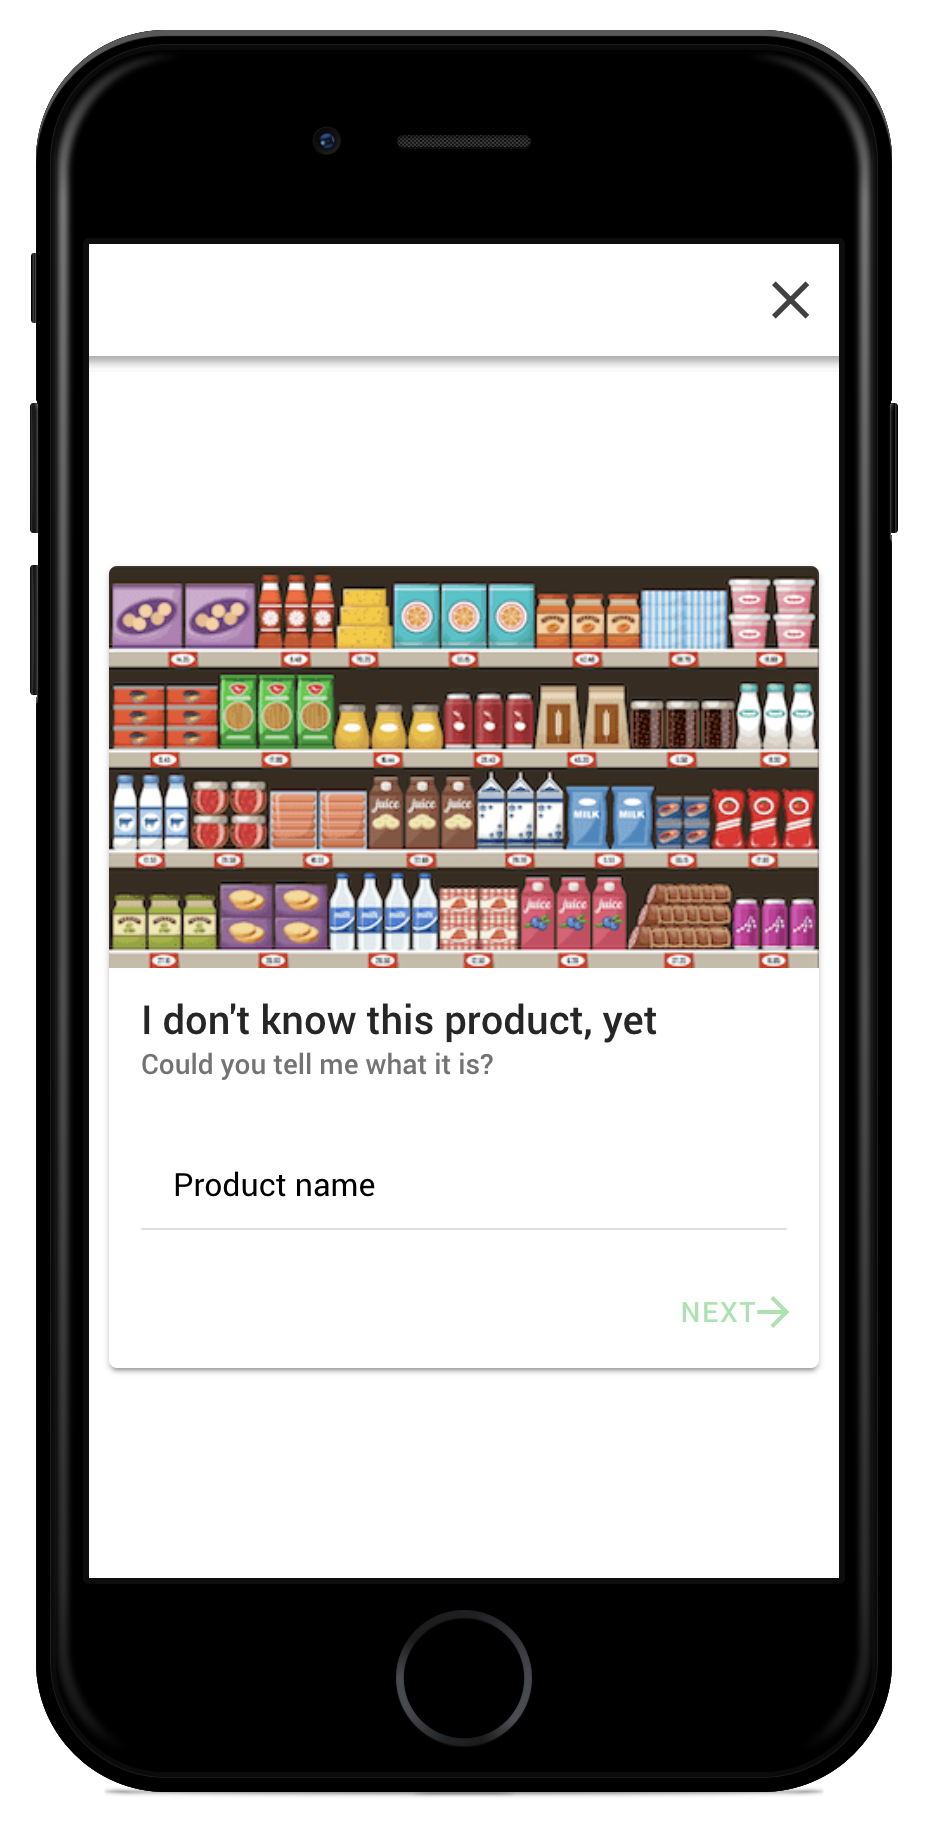
\includegraphics[width=\textwidth]{capture-0}
         \caption{Name capture}
         \label{fig:capture-0}
     \end{subfigure}
          \hfill
     \begin{subfigure}[b]{0.28\textwidth}
         \centering
         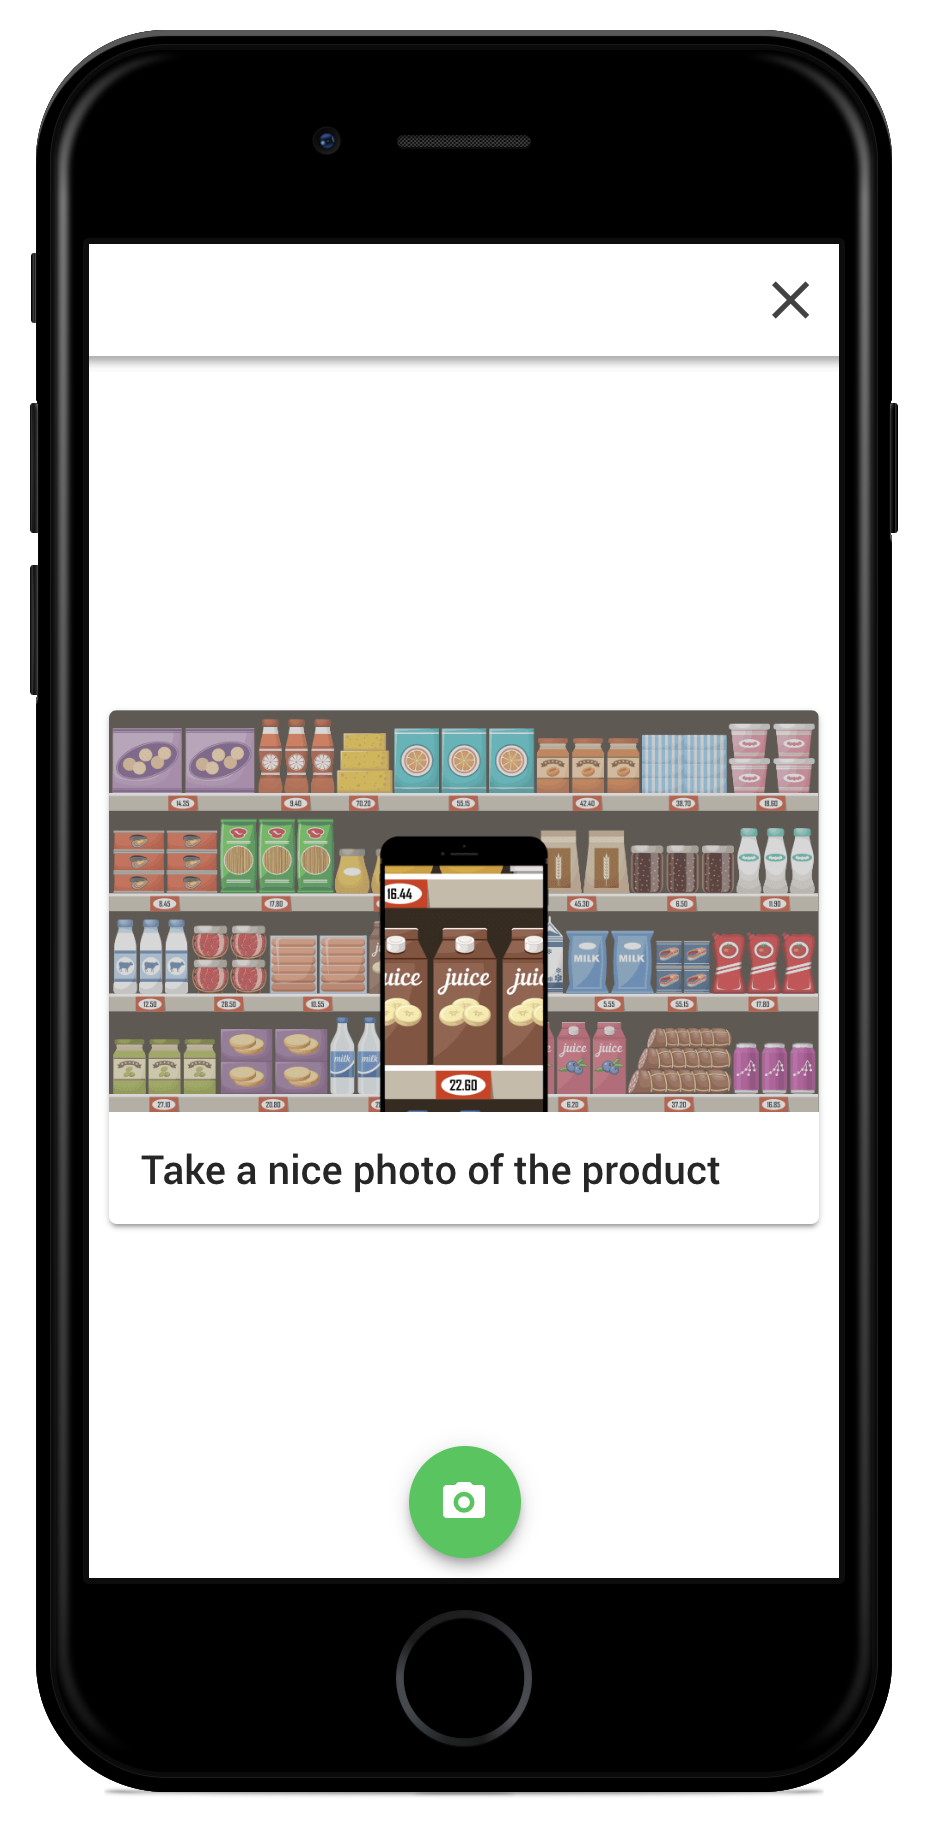
\includegraphics[width=\textwidth]{capture-1}
         \caption{Photo capture}
         \label{fig:capture-1}
     \end{subfigure}
          \hfill
     \begin{subfigure}[b]{0.28\textwidth}
         \centering
         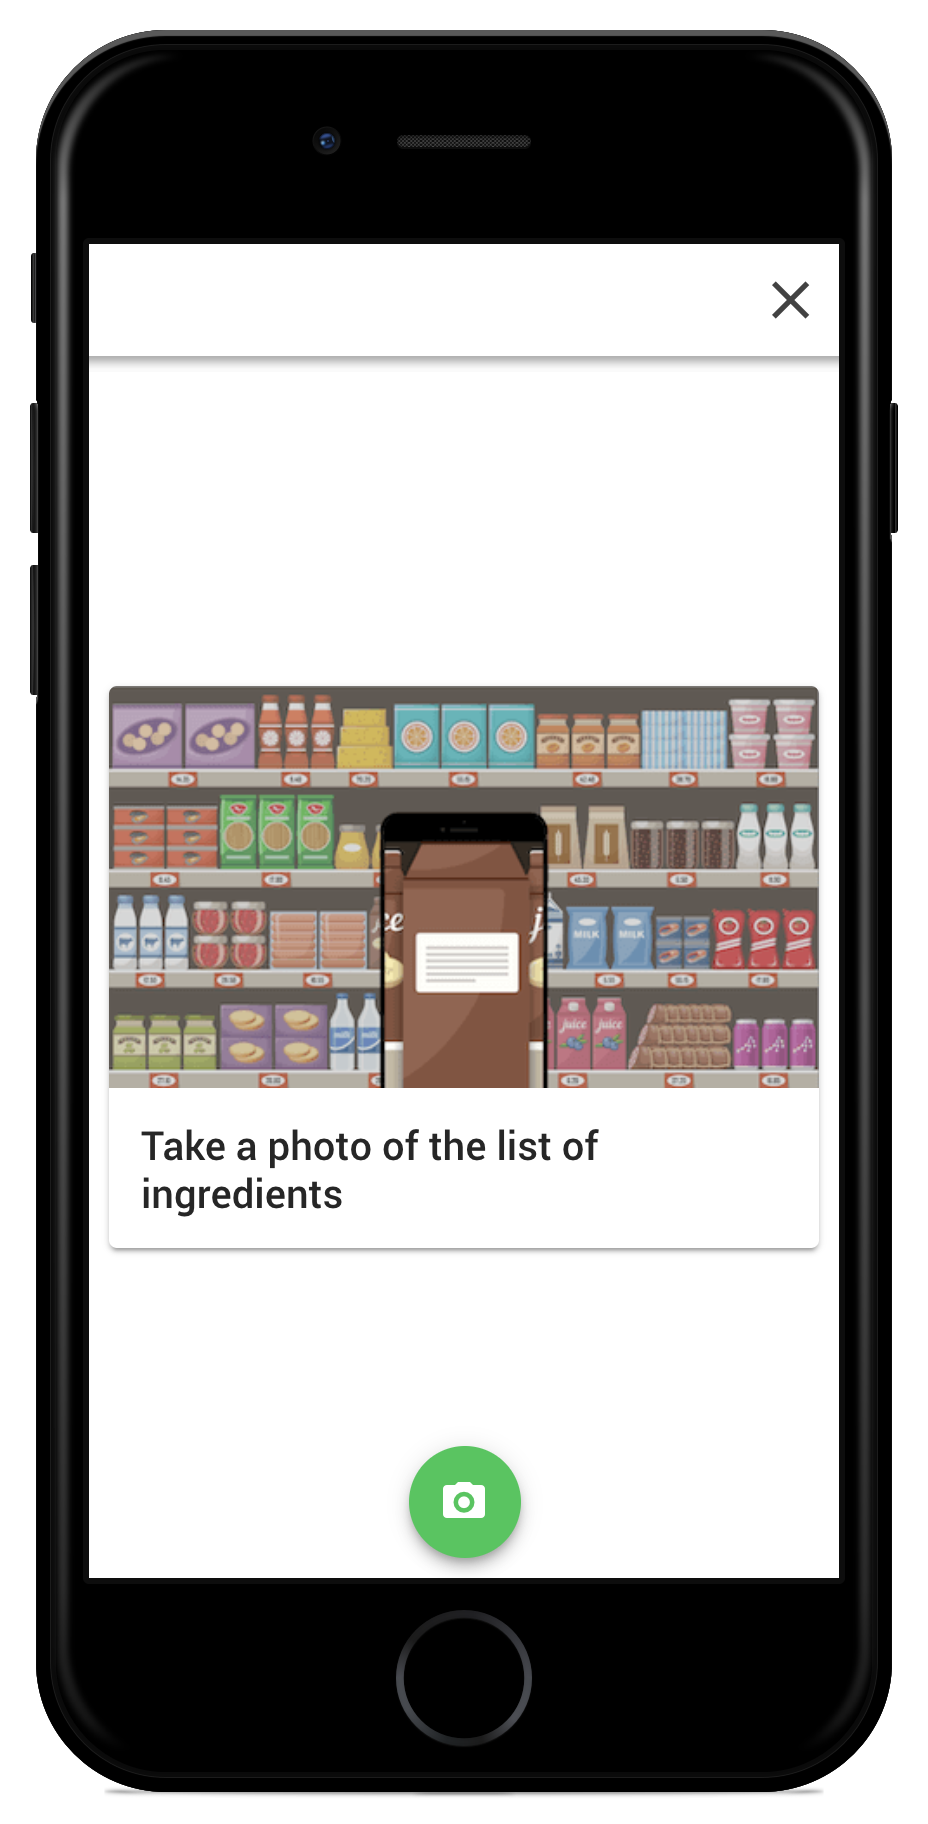
\includegraphics[width=\textwidth]{capture-2}
         \caption{Label capture}
         \label{fig:capture-2}
     \end{subfigure}
        \caption{Product capture}
        \label{fig:capture}
\end{figure}

\subsection{Feedback Survey}
\label{sub:feedback-criteria}

As soon as the user has successfully scanned at least three distinct products on two different days, a feedback survey is triggered. The survey contains ten questions, which can be found in \cref{chap:feedback-schema}.

\begin{figure}[H]
     \centering
     \begin{subfigure}[b]{0.32\textwidth}
         \centering
         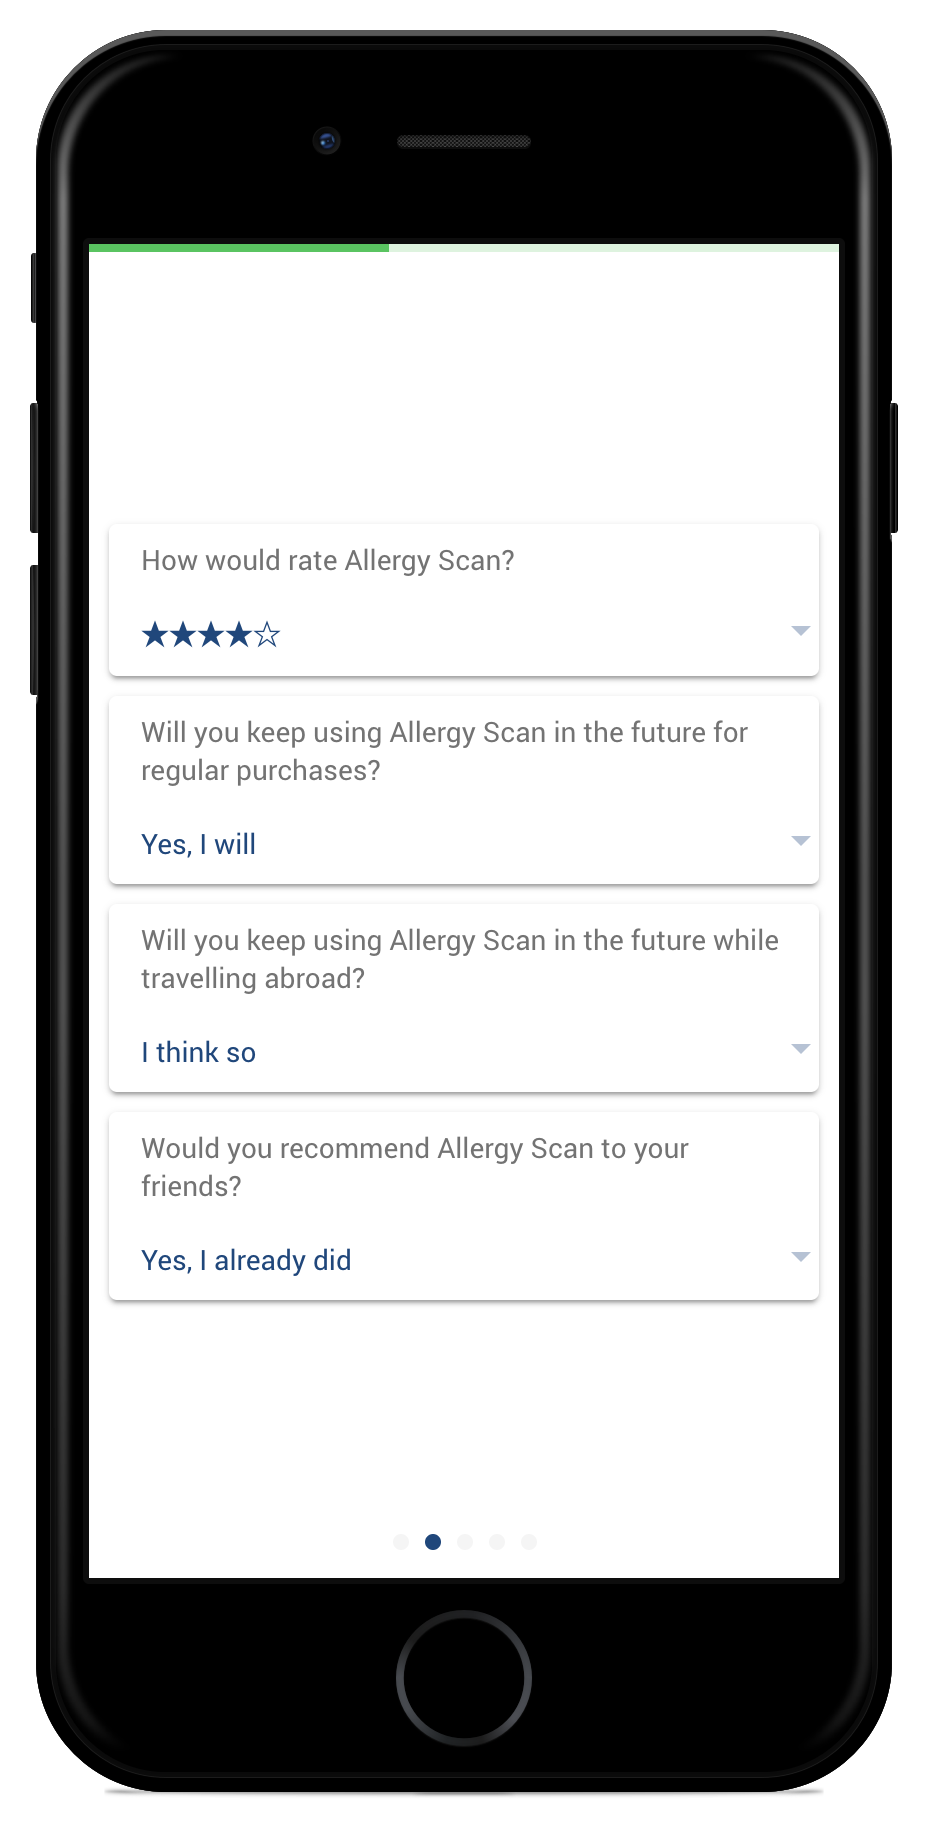
\includegraphics[width=\textwidth]{feedback-1}
         \caption{Intention to use}
         \label{fig:feedback-1}
     \end{subfigure}
          \hfill
     \begin{subfigure}[b]{0.32\textwidth}
         \centering
         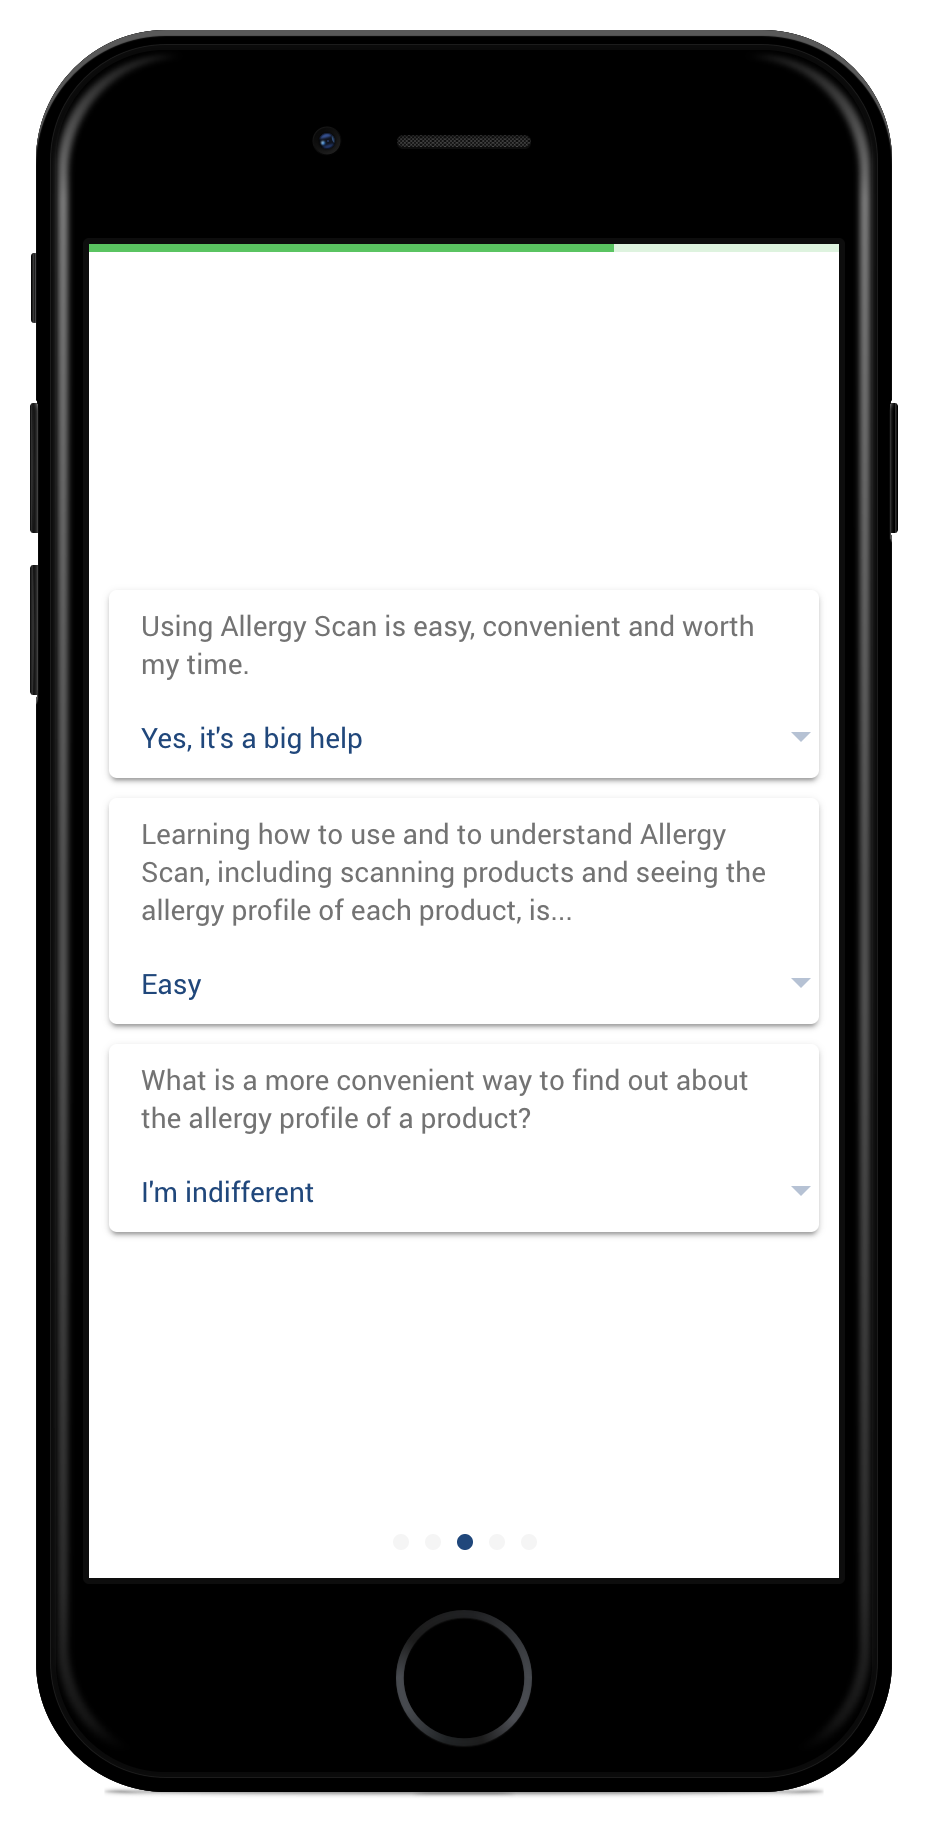
\includegraphics[width=\textwidth]{feedback-2}
         \caption{Effort expectancy}
         \label{fig:feedback-2}
    \end{subfigure}
          \hfill
     \begin{subfigure}[b]{0.32\textwidth}
         \centering
         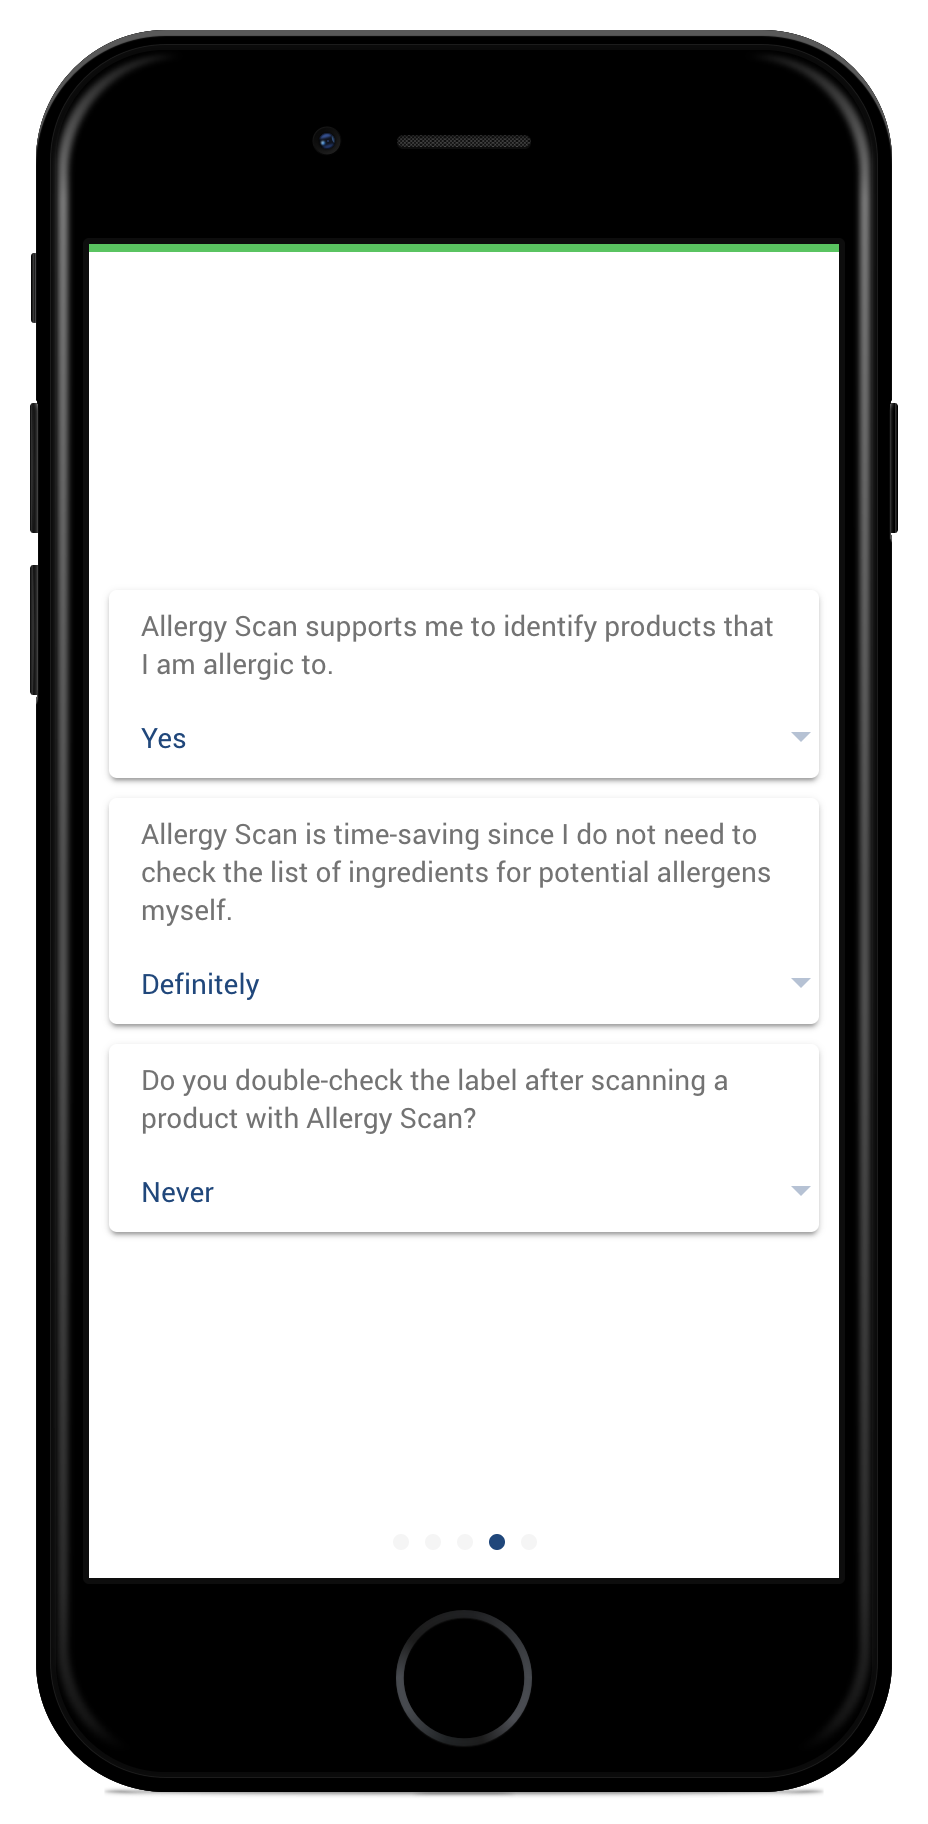
\includegraphics[width=\textwidth]{feedback-3}
         \caption{Performance expectancy}
         \label{fig:feedback-3}
     \end{subfigure}
        \caption{Feedback form}
        \label{fig:feedback}

\end{figure}


\section{Architecture}

\subsection{Frontend}
Angular is a modern JavaScript framework maintained by Google \citep{angular} which allows developers to build web application using the latest technologies of the current web standards. The probably most important feature of \emph{Allergy Scan} is to access the device's camera for the purpose of scanning bar codes and taking photographs of the products. Currently, however, this was only achievable with native applications \citep[28]{jobe_2013} as the overall browser support for accessing the camera of a mobile device using web standards was not sufficient enough, yet \citep{takePhoto}.\\

Thus, Angular alone is not sufficient in this case and therefore the Ionic framework \citep{ionic} had to be included in this study. Ionic is built on top of the Angular framework and enables developers to compile an application written in web technologies to a mobile application for iOS and Android devices. This can be attained with the help of a Cordova \citep{cordova} wrapper, which allows the application to extend the access to features, such as the camera and build a hybrid app \citep[29]{jobe_2013} ready to be published in the App Store and Google Play Store.

\subsection{Backend}
Firebase is a Backend-as-a-Service and is used to run \emph{Allergy Scan}'s background functionality. More precisely, Firestore, a real-time NoSQL database, enables the storage of all data which is required and generated by the application, such as the configuration of each user, all executed product scans and their result and the captured user feedback. Moreover, Firebase's Cloud Functions serve as a proxy server between the application and the Eatfit API.

\subsection{Product Data Service}
\label{sub:eatfit}

The product data is provided by a RESTful API called \emph{Eatfit}. Eatfit is maintained by the Auto-ID Labs and retrieves information on a product, such as images, list of ingredients and contained allergens through a product’s bar code. As several existing databases are merged into Eatfit, namely Codecheck, Openfood, Open Food Repo and Trustbox, users of Eatfit have access to information on several hundred thousand products. At the present moment, three other applications from the Auto-ID Labs rely on Eatfit as well.